%new commen
\documentclass[11pt,epic,leqno,eepic,psfig,]{article}
%\usepackage{soda-good}
\usepackage{amsmath}
\usepackage{amssymb}
\usepackage{graphicx}
\graphicspath{ {images/} }
%\usepackage{epsfig}
%\usepackage{psfig}
\usepackage{subfigure}
%\usepackage{url}
%\usepackage{picins}
\usepackage{color}
\usepackage{alg}

 \usepackage[dvipsnames]{xcolor}


 \usepackage[bindingoffset=0.2in,%
            left=1in,right=1in,top=1in,%bottom=4in,%
            footskip=.45in]{geometry}



\newcommand{\rbox}{\begin{flushright}
        \vspace{-8mm}
        \qed
        \vspace{-1mm}
        \end{flushright}
}

%%%%%%%%%% Change \ans to using \newenvironment answer %%%%%%%%%%
\def\NULL{\color{brown}\mbox{\sl NULL}}
\def\AND{{\color{brown}\mbox{\bf AND}}}
\def\OR{{\color{brown}\mbox{\bf OR}}}
\def\while{{\color{brown}\mbox{\bf while}}}
\def\iff{{\color{brown}\mbox{\textbf{If}}}}
\def\for{{\color{brown}\mbox{\textbf{for}}}}
\def\return{{\color{brown}\mbox{\textbf{return}}}}

% \newenvironment{ans}{\color{brown}
%   \slshape
%   \vspace{1pt}
%   \textbf{Answer:}
%   \vspace{3pt}
%   \newline
% }
% {
%   \vspace{3pt}
%   \normalfont\color{red}
% }


\newcommand{\ans}[1]{{\color{brown}{\bf\Large Answer:} \sl  #1 \color{black}}}



\newcommand{\commentout}[1]{{}}
\newcommand{\ceil}[1]{\left \lceil #1 \right\rceil}

%%%%%%%%%%%% Comment these two if this isn't the solution %%%%%%%%%%%%%%%%%%%
%\newcommand{\ans}[1]{{ {\Large Answer} {#1}  }}





\newcommand{\isSol}[2]{#2}      % Display second parameter, but not first

%%%%%%%%%%% Comment these two if this isn't the solution %%%%%%%%%%%%%%%%%%%%%%

%\newcommand{ans}{}
%\newcommand{\isSol}[2]{#1}    % Display first parameter, but not second

%%%% newcommand for displaying formulas with less vertical whitespace %%%%

\newcommand{\df}[1]{
  \vspace{-5pt}#1\vspace{-15pt}
}


\renewcommand{\i}{\item}


\isSol{\pagesytle{empty}}{\pagestyle{plain}}
\newcommand{\figlab}[1]{\label{fig:#1}}
\newcommand{\figref}[1]{Figure \ref{fig:#1}}
\def\marrow{{\marginpar[\hfill$\longrightarrow$]{$\longleftarrow$}}}
   \def\alon#1{{\sc Alon says: }{\marrow\sf #1}}
\def\eps{\varepsilon}
\def\B{{\cal B}}
\def\T{{\cal T}}
\def\D{{\cal D}}
\def\Cov{\mbox{\sl Cov}}
\def\bt{\beta}
\def\al{\alpha}
\newcommand{\comm}[1]
{\marginpar{$\longleftarrow$}$\,\mbox{}^{\rm com}${\sf #1}$\mbox{}_{\rm ment}\,$}

\newcommand{\Fr}{Fr\'{e}chet\ }
\newcommand{\Frd}{Fr\'{e}chet distance\ }
\newcommand{\f}{\ensuremath{d_F}}
\newcommand{\wf}{\ensuremath{d_{\tilde{F}}}}
\newenvironment{proofsketch}{{\bf Proof Sketch:}}{{\rbox}}
\newtheorem{prop}[section]{Proposition}
\newtheorem{Def}[section]{Definition}
%\newtheorem{claim}[section]{Claim}

%\newtheorem{lemma}{Lemma}[section]
%\newtheorem{theorem}[lemma]{Theorem}

%\newtheorem{theorem}{Theorem}[section] % section
%\newtheorem{lemma}[section]{Lemma}
%\newtheorem{corollary}[theorem]{Corollary}
%\newtheorem{example}[theorem]{Example}
%\newtheorem{defn}[theorem]{Definition}
%\newtheorem{question}[theorem]{Question}



%\topmargin 3mm \textwidth 6.4 in \oddsidemargin +0.19in \evensidemargin +0.19in
%\textheight 8.5in \textwidth 6.0 in \columnsep .33in \columnseprule 0pt
\parskip=0.7mm
\headsep 3mm



\newcommand{\euclidean}{{\Bbb E}}
\newcommand{\reals}{{\Bbb R}}
\newcommand{\sphere}{{\Bbb S}}
\newcommand{\integers}{{\Bbb Z}}
\newcommand{\naturals}{{\Bbb N}}
\newcommand{\complex}{{\Bbb C}}
\newcommand{\rationals}{{\Bbb Q}}
\newcommand{\seg}[1]{\overline{#1}}
\def\TP{{\sl TP}\ }
\def\S{{\cal S}}
\def\maxs{{\sl max}(\sum}
\def\maxs{{\sl max\_}\sum}
%\def\sum{\mbox{\sl sum}}
\def\F{{\cal F}}
\def\epsilon{\varepsilon}
\def\Pos{{\sl Pos}}
\def\Neg{{\sl Neg}}
\long\gdef\boxit#1{\vspace{5mm}\begingroup\vbox{\hrule\hbox{\vrule\kern3pt
\vbox{\kern4pt#1\kern3pt}\kern3pt\vrule}\hrule}\endgroup}
\newcommand{\qed}{\mbox{}\hspace*{\fill}\nolinebreak
 \mbox{$\rule{0.7em}{0.7em}$}}


 %\newsymbol\subsetneqq 232A
 %\newsymbol\nsubseteq 232A
\newcommand{\comment}[1]{}
\newcommand{\ToAppear}[1]{\raisebox{15mm}[10pt][0mm]{\makebox[0mm]{\makebox[\textwidth][r]{\emph{#1}}}}}


\title{ CSc545 - fall 2018 - Homework \#1. \\
 Due:  Sep 22  2018  11:59pm \\ Jordan L. Siaha}

\vspace{-10mm}

\begin{document}
\maketitle







%\isSol{
\fbox{
\begin{minipage}{6 in}
\textbf{Instructions.}
\begin{enumerate}

\i Solution may {\bf not} be submitted by students in pairs.

\i You may submit a pdf of the homework, either printed or hand-written and scanned, as long as it is {\bf easily} readable.

\i If your solution is illegible not clearly written, it might not be graded.

\i Unless otherwise stated, you should prove the correctness of your answer. A correct answer without justification may be worth less.

\i If you have discussed any problems with other students, mention their names clearly on the homework.
These discussions are not forbidden and are actually {\bf encouraged}.
However, you must
write your whole solution yourself.

\i Unless otherwise specified, all questions have the same weight.

\i  You may refer to data structures or their properties studied in class without having to repeat details, and may reference theorems we have studied without proof. If your answer requires only modifications to one of the algorithms, it is enough to mention the required modifications, and the effect (if any) on the running time and on other operations that the algorithm performs.


\i  In general, a complete solution should contain the following parts:
\begin{enumerate}
\i A high level description of the data structures (if needed).  {\sl E.g. We use a binary balanced search tree.
Each node contains, a  key and pointers to its children. We augment the tree so each node also contains a field... }
\i A clear description of the main ideas of the algorithm. You may include pseudocode in your solution, but this may not be necessary if your description is clear.
\i Proof of correctness (e.g. show that your algorithm always terminates with the desired output).
\i A claim about the running time, and a proof showing this claim.
\end{enumerate}
%\i \textcolor{blue}{When talking about tress, do not confuse the
% {\em children} of a node  with the {\em decedents} of the node. }
\end{enumerate}
\end{minipage}

 }




\renewcommand{\i}{\item}


 \everymath{\color{blue}}


\def\polylog{{{\sl polylog }}}
\def\poly{{{\sl poly }}}


%Due Time: 2/15/05

%Turnin ID: $cs352\_assg2$

%Turnin files: Qremove.c, ExponentCheck.c, sum.c

\newpage







\begin{enumerate}



 


\i Consider an infinite sequence of functions $f_i$. It is known that for every $i$, it is true that $f_i (n)=O(n)$. We define a new function
$g(n)=\sum_{i=  1} ^n f_i(n)$. Is it true than $g(n)=O(n^2)$ ?

\ans{\Large We can rewrite this as a summation series: \\$g(n)=f_1(n) + f_2(n) + f_3(n) +... + f_n(n)$
\\And we know that $f_i (n)=O(n)$, \\so we can replace every  $f_i (n)$ with $O(n)$, \\so we get $g(n)=\sum_{i=  1} ^n O(n)$ \\and from the arithmetic series
defined for insertion sort in the slides, it would be valid to say that  $g(n)=O(n^2)$ }
 \\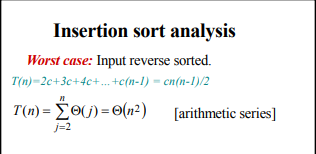
\includegraphics{insertionSort}

\i Assume that we insert the keys $1,2\dots n$ into a binary search tree $T$.
The algorithm for inserting a key $k_i$ is simple. Initially the tree is empty. Then for $i=1,2\dots n$,  to insert key $k_i$   we perform a search for $k_i$ starting  at the root of $T$,  %perform {\tt search $k_i$},
and once reaching a NULL pointer, we insert $k_i$ as a new leaf. For simplicity, assume $k_i=i$.

We do {\bf not }not balance the tree after each insertion.

As usual $h(T)$,  the height of $T$  denote the number of edges from the root of $T$ to the leaf that is the most remote from the root.


\begin{enumerate}
\i warm-up
\begin{enumerate}
    \item show that the height of $T$ is $\Theta(n).$
\\\ans{Since it is given that the keys are inserted in increasing order from $1-n$, this means that for every insert, the current key we are trying to insert is greater than the previous key
	that was inserted, therefore, every key inserted would forcefully end up being the right node of the previous key inserted and our tree height would grow by $1$ for every insert,
	turning our tree into what is essencially a list. Therefore, the tree height of  $T$ is $\Theta(n).$}
    \i Show that the time to perform all $n$ insertions is $\Theta(n^2)$
\\\ans{If we imagine the tree as a list again as in the previous answer, we can also assume the properties of a list when inserting into this tree given that every $k_i = i for$ $i = 1, 2\dots n$
\\ This means that the insert operation in this tree takes $\Theta(n)$ since we are always inserting at the end of our imagined list.
\\ We can therefore write a function $g(n)$ that represents all insert operations in this tree and write it as the summation:
\\  $g(n)=\sum_{k_i=  1} ^n \Theta(n)$ which is the same as $g(n) = \Theta(n^2)$}
    \i next we insert the same keys into $T$ but we could pick different permutations.  Show that there is an order for which the time to perform all insertions is $O(n\log n)$
\\\ans{First, we need to use the assumption that the keys are given in the order from $1, 2, ... n$(A sorted order) to our advantage.
\\ This means that BEFORE we pick any keys to insert, we have an array of numbers going from $1, 2... n$
\\ Using this fact about the numbers, we can perform a binary search style search on the keys to grab the middle element of each of the partitions of each binary search step.
\\ This can be done because binary search splits the given array into 2 partitions using the middle element, yielding two partitions such that every element in the left partition is smaller
than the middle element and every element in the right partition is bigger than the middle element.
\\ This is important because if we were to choose such middle elements until all elements in the initially sorted array are chosen, then inserting these middle elements while keeping the order
in which they were selected into the binary search tree would create a tree of height $log(n)$ because every key chosen would have a left and a right child if there were at least 3 elements
in each sub-partition array.
\\ By picking the middle element in each sub-partition array, we force all elements smaller than it to the left and all elements bigger than it to the right and repeat the process for every element. This should split the tree into 2 subtrees and we do this $n$ times for all elements, therefore, each insertion takes maximum $log(n)$ or $O(log n)$ and we have $n$ insertions, to
perform, yielding a total of $O(n log n)$ time to perform all insertions.}
    \i  During the process of constructing the tree, we define random variable $Y_{ij}$ to be 1 iff the keys $i$ and $j$ were compared to each other. (For every $1\leq i, j\leq n.$)
    Otherwise $Y_{ij}=0.$ Show that the work to construct the tree is proportional to
    $$\sum_{1\leq i,j\leq n} Y_{ij}.$$

    For example if $j$ is the first key that was inserted, then it is in the root of $T$ and it is compared to every other key inserted afterward.

    \end{enumerate}
   \i Next assume that the keys are inserted in a random order, where each permutation is equally likely.
    \begin{enumerate}

    \i  What is the expected time $$E\left(\sum_{1\leq i,j\leq n}Y_{ij}\right) ? $$
    \i Prove  that the expected distance of a key $j$ from the root is $O(\log n)$
    \i Prove that for large enough {\bf  constant}  $c$, and large enough value of $n$, the probability that $h(T)\leq c\log_2n $ is very close to 1.
    You could pick what is $c$ and how to formalize 'close to 1'

    \end{enumerate}




\end{enumerate}



\i Show the preference list of a set of $n$ men and $n$ women, for which more than one single stable pairing exists.

\ans{We can consider the following preference lists for 3 men and 3 women
\\$M_1$ : \textcolor{red}{W1}, \textcolor{red}{W2} , \textcolor{red}{W3}  -----  \textcolor{red}{W1} : $M_1$; $M_2$; $M_3$
\\$M_2$ : \textcolor{red}{W1}, \textcolor{red}{W3} , \textcolor{red}{W2}  -----  \textcolor{red}{W2}  : $M_2$, $M_3$, $M_1$
\\$M_3$ : \textcolor{red}{W2}, \textcolor{red}{W3} , \textcolor{red}{W1}  -----  \textcolor{red}{W3}  : $M_3$, $M_1$, $M_2$
\\Since $M_1$ and  \textcolor{red}{W1}  are at the top of each others' preference lists, they will be matched with each other in any stable pairing to prevent them from going rogue.
\\That leaves any combination of the rest of the two couples where Both $M_2$ and $M_3$ can be matched to either \textcolor{red}{W2} or \textcolor{red}{W3} without rogue couples.
\\ This gives us the following 2 stable pairings:
\\ P1 = ($M_1$, \textcolor{red}{W1}), ($M_2$, \textcolor{red}{W3}), ($M_3$, \textcolor{red}{W2})
\\ P2 = ($M_1$, \textcolor{red}{W1}), ($M_2$, \textcolor{red}{W2}), ($M_3$, \textcolor{red}{W3})}

 \i Suggest an $O(n^2)$-time algorithm that determines if, given the preference lists of all the men and women, there exists more than one stable matching.

  \i Suggest a modification of the SkipList structure, such that in addition to the operations
 { \tt insert$(x)$, find$(x)$ } and {\tt delete$(x)$}, you could also answer the operation {\tt $avg(x_1, x_2)$ } which reports the average of all keys stores in the skip list whose value is $\geq x_1$ but $\leq x_2$.
 The {\em expected}  time for each operation should be $O(\log n)$.


Hint: Start by  storing  at each node $v$ of the SL another field, called {\sl size}$[v]$, containing the number of keys in the SL between $v$ and the next node at the same level as $v$. Note that maintaining the values of these fields might imply extra work while performing other operations.




\i
\begin{enumerate}

\i  Let $d$ be a fixed positive integer.
Next consider a perfect SkipList constructed  as follows:  In order to create the $i$th level $L_i$ of the SkipList, we scan the  keys  of  level $L_{i-1}$, and promote to $L_i$ every {\bf d'th} key.
So for example, the perfect SkipList discussed in class uses the value $d=2$. The case   $d=3$ implies that every third key is promoted, and so on.
\begin{enumerate}

\i What exactly is the worst case running time of {\tt find}$(x)$, as a function of both $d$ and $n$ ?

\i   Which  value(s) of $d$ will do you think would lead to  good performances, and which are poor choices? Why?


\end{enumerate}


\i In this question, consider a SkipList ${\cal L}$  created by inserting a set $S$ of $n$  keys into an (initially empty) SkipList.  As seen in class, if a key $x$ appears in level $i$, the probability that it also appears in level $i+1$ is $\frac {1}{2}$.

Assume that we re-create a SkipList by inserting the same keys, in the same order, but this time this probability $p$ is $0.01$.  (if a key $x$ appears in level $i$, the probability that it also appears in level $i+1$ is $0.01$.    ) Will the expected time to perform
{\sl find$(x)$} operation increase or decrease, compared to the expected time for the same operation in the original SkipList ${\cal L}$ ?



\end{enumerate}





 \i

 What is the expected value of $cnt$ after the following function is executed ?

\fbox{
 \begin{minipage}{9.5in}
    \baselineskip 1mm
    \begin{tabbing}
       \hspace{6mm}\=\hspace{6mm}\=\hspace{6mm}\=\hspace{5mm}\=\hspace{5mm}\=\hspace{5mm}\=\hspace{5mm}\=\hspace{5mm}\=\hspace{5mm}\=\hspace{5mm
}\=\hspace{5mm}\= \kill
 $cnt=0; M=-\infty $ ; \\
 for $i=1$ to $n$ \{ \\
 \> $x_i =rand()$  ; {\color{brown} Comment:  returns a random {\bf float} number of between $0$ and $1$. } \\
 \> if $(x_i>M)$ then \{ \\
 \>\>$M = x_i $; \\
 \>\> $cnt++ $;  \\
 \> \} \\
  \}
 \end{tabbing}
\end{minipage}
}\\


Hint: Define the random variable $Y_i$ which is $1$ if
$$x_i > \max\{x_1, x_2\dots x_{i-1}\} $$
and $Y_i=0$ otherwise. What is
$E(Y_1+Y_2+\dots + Y_n )$.

\ans{If we define the variable $Y_i$ which is 1 if $x_i > \max\{x_1, x_2\dots x_{i-1}\} $, then on the first iteration of the loop, this variable is guaranteed to be 1 since anything is bigger than negative infinity, so count is at least one from the beginning. This means that $Y_i$ is 1.
\\ For the next iterations of the loop, we're going to choose some number between 0 and 1, and whatever number we choose, we divide all numbers between 0 and 1 into 2 partitions using the random number between 0 and 1 that we got as reference point. One side of the partition represents $Y_i = 0$ or $Y_i = 1$.
\\ If we assume that we get a nice even spread of random numbers, then each side that the random number lands on should be roughly $log(n)$, because the odds of getting something higher than what we got last time is proportional to how many divisions(which side) in we are. In an arithmetic sequence, assuming the nice even spread of numbers, this would look something like: 
\\ $1 + \frac{1}{2} + \frac{1}{4} +\frac{1}{8}...+ \frac{1}{n} = log(n)$ 
\\ Therefore, the expected value of $cnt$ is $log(n)$. }





\i  Create a SkipList for a set of $n$ keys
$S=\{k_1\dots k_n\}$.
The keys are known in advance, and are sorted. The height of the Skiplist is $\leq 3$.

The SkipList should be designed such that $$\max_{k_i\in S} T(k_i) $$ is as small as possible, where $T(k_i)$ is defined as the time for searching $k_i$, where the search is starting, as usual in the upper leftmost element.





\i Let $L$ be a perfect SkipList constructed on a set of $n$ keys, and let $X=\{k_1\dots k_m\}$ be another  set of keys. Assume $m<n$.  Suggest an $O(m\log({\frac {n }{m}}))$ time  algorithm for computing which key(s) of $X$  appear in $L$.  {\color{brown} You could assume that $X$ is sorted}.



You could {\bf not } assume that the keys of $X$ are equally spaced in $L$. Yet understanding this special case could shed some intuition.

\end{enumerate}


\end{document}
